\documentclass[12pt]{article}
%\documentclass{article}

\usepackage{times}
\usepackage[final]{graphicx}
\usepackage{hyperref}
\usepackage{verbatim}

\setlength{\topmargin}{-0.5in}
\setlength{\oddsidemargin}{0in}
\setlength{\evensidemargin}{0in}
\setlength{\textwidth}{6.5in}
\setlength{\textheight}{9.0in}

\begin{document}

\centerline{\bf \Large CS295/CS395/CSYS395: \href{CS295_395_Syllabus.pdf}{\underline{Evolutionary Robotics}}}

\vspace{0.5cm}

\centerline{\bf \large Programming Assignment 4 of 10}

\vspace{0.5cm}

\centerline{\large Assigned: Friday, September 23, 2011}

\vspace{0.5cm}

\centerline{\large Due: Friday, September 30, 2011 by midnight}

\vspace{0.5cm}

\noindent \textbf{Description:} In this assignment you will download, install and make some changes to the Bullet Physics Library, the open source physics engine we will be using for the remainder of this class. After installation and compilation, you will run a test application that comes with Bullet which simulates a vehicle (Fig. \ref{Fig}a). You will then change the radii of the wheels in the Bullet code, re-compile and re-run the code to produce Fig. \ref{Fig}b. You will then comment out all the Bullet code that creates, simulates and draws the objects and joints in this example program, producing the `empty world' shown in Fig. \ref{Fig}c. This will provide you with a blank canvas on which you will begin to build your robot in the next assignment. \\

\noindent \textbf{Important:} If you get stuck installing Bullet, get on the Bullet forum and ask your question; you will usually get a response in a couple of hours. \textbf{This means of course that you will have to start the assignment before the night before.} If you are still stuck, come see the instructor or teaching assistant.

\begin{enumerate}

\item \textbf{Back up your Python code from last week.} If you lose your laptop tomorrow, will you still have your code from assignments 1-3?

\item Download Bullet version 2.79. Download instructions can be found on Bullet's
\href{http://bulletphysics.org/wordpress/}{\underline{main page}}. Make sure to download from \href{http://code.google.com/p/bullet/downloads/list}{\underline{code.google.com}}.

\item Upzip the archive.

\item \textbf{If you are working on a Mac or on Linux}, follow the installation instructions found in INSTALL. Once installed, skip to step~\ref{post-install}.

\item Skipping windows specific installation steps for the moment.
\begin{comment}

\item \textbf{If you are working on Windows}, installing Bullet is a bit trickier. Download and install the free C++ compiler
\href{http://www.softpedia.com/get/Programming/Other-Programming-Files/Microsoft-Visual-C-Toolkit.shtml}
{\underline{Visual C++ 2005 Express Edition}}. \textbf{Note from the T.A.:} There is a 2010 version of Visual C++ that is free from Microsoft. Visual Studio 2010 Express (includes C++).

\item Download and install \href{http://www.microsoft.com/downloads/en/details.aspx?FamilyId=0BAF2B35-C656-4969-ACE8-E4C0C0716ADB&displaylang=en}
{\underline{Windows Server 2003 Platform SDK}}. \textbf{Note from the T.A.:} There is an update to Windows Server 2003 Platform SDK which supports Windows 7, and earlier Windows versions including Vista and XP. Windows SDK for Windows 7 and .NET Framework 4


\item Open a Windows Command Prompt (in Windows XP, Start$\rightarrow$Run...$\rightarrow$cmd[enter]), and navigate to ode-0.11.1/build.

\item type \texttt{premake4 --with-demos --with-tests vs2005}

\item Close the Command Prompt and doubleclick on ode-0.11.1/build/vs2005/ode.sln, which will open ode, drawstuff (the drawing routines) and all of the demos in Visual C++.

\item in Visual C++ go to Tools/Options/Projects and Solutions/VC++ Directories.

\item Select `Show directories for'/Executable files, and add a directory pointer to \\
\texttt{C:/Program Files/Microsoft Visual Studio 8/VC/Microsoft Platform SDK for Windows Server 2003 R2/Bin}.

\textbf{Note from the T.A.:} VC++ Directories editing in Tools$\rightarrow$Options has been deprecated; directories are now available as a user property sheet that is added by default to all projects. Had to edit the output directory name in the linker property sheets for drawstuff and ode.

\item Select `Show directories for'/Include files, and add a directory pointer to \\
\texttt{C:/Program Files/Microsoft Visual Studio 8/VC/Microsoft Platform SDK for Windows Server 2003 R2/Include}

\item Select `Show directories for'/Library files, and add a directory pointer to \\
\texttt{C:/Program Files/Microsoft Visual Studio 8/VC/Microsoft Platform SDK for Windows Server 2003 R2/Lib}

\item Now Select Build/Build Solution to compile Bullet, drawstuff and all the demo programs.

\end{comment}
\item \label{post-install} For windows users you should now find executables of the demo
  programs in \\ \texttt{ode-0.11.1/lib/debugdoubledll}. For Linux and
  Mac users, you should find the executables in
  \texttt{bullet-2.79/Demos/RagdollDemo}. Run the RagdollDemo
  executable.

\item You should see something like in Fig. \ref{Fig}a. Try familiarizing yourself with the commands given in Table~\ref{commands}. Screencapture the simulation window, and paste the result into your document.

\begin{table}[h]   \begin{center}
    \begin{tabular}{ | l | l | }
      \hline
      Key & Description \\
      \hline
      l,r,f,b & Move camera left, right, front, or back \\
      z,x & Zoom in or out \\
      e & Add another ragdoll to the simulation \\
%      i & Toggle idle \\
      g,u & Toggle shadows, and textures \\
      h & Toggle debug text \\
      w & Draw wireframes and body reference frames \\
%      p & Toggle profile timings \\
%      m,n,t,y & Toggle sat comparison, LCP, draw text, draw features \\
      a & Draw Axis Aligned Bounding Box (AABB) \\
      c & Draw contact normals (black lines) \\
      C & Draw contraints \\
      L & Draw contraint limits \\
      d & Disable body deactivation  \\
%      o & Orthographic projection  \\
      space & Reset scene \\
%      1 & Toggle CCD mode
      . & Shoot box (or right-click) \\
      +,-& Increase or decrease box speed\\
      left-click-and-drag & Drag a body part \\
      q & Quit application \\
      \hline
    \end{tabular}
  \end{center}
  \caption[Short name]{\label{commands}Brief list of key commands for
    Bullet demo applications}
\end{table}

\item Open the code for RagdollDemo, and find the line that specifies the radii of the capsule that represents the head. Multiply those radii by four to produce ragdolls that look like bobble-head toys, recompile, and re-run the demo. Screencapture the simulation window  (which should look like Fig. \ref{Fig}b) and paste the result into your document.

\item \label{turn-off-sim} Now you will allow the application to create data structures and draw objects, but not run the physics simulation.  Comment out this line of code in RagdollDemo.cpp in RagdollDemo::clientMoveAndDisplay(): \\
\texttt{ m\_dynamicsWorld->stepSimulation(ms / 1000000.f);} \\
Re-compile and re-run to ensure the program still starts and ends without crashing.  Note: the ragdolls should not fall as they did before and clicking on them does not cause them to move.

\item Let's remove one ragdoll from the simulation.  Find the function RagdollDemo::initPhysics() and comment out the second to last line: \\
\texttt{	spawnRagdoll(startOffset);} \\
Re-compile and re-run.  Only one ragdoll should be shown and the physics simulation should still be off, so it won't fall.  Screencapture the simulation window (which should look like Fig. \ref{Fig}c) and paste the result into your document.

\item Re-enable the physics simulation by uncommenting the stepSimulation function call we did in Step~\ref{turn-off-sim}, so that that the ragdoll falls to the ground when RagdollDemo is executed.

\item Now you will allow an `empty' simulation to run.  Comment out the other call to spawnRagdoll() in initPhysics().  Confirm that no ragdolls are shown.  Re-compile, re-run and ensure that the program still starts and ends without crashing.

\item Recompile, re-run, and you should get an empty simulation as shown in Fig. \ref{Fig}c. Screencapture the window and copy it into your document.

\item Submit your document (containing four images) in .pdf format to the Teaching Assistant.

\end{enumerate}

\begin{figure}[!t]
\centerline{
a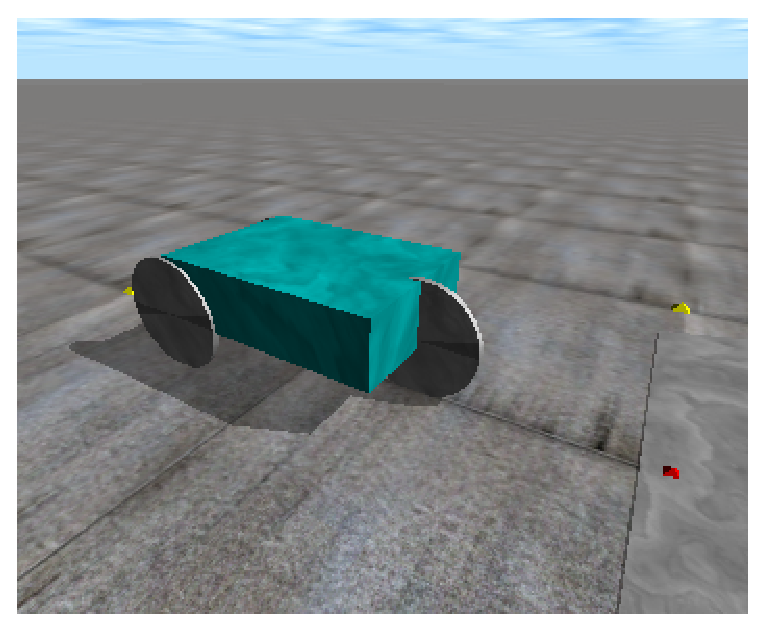
\includegraphics[width=0.48\textwidth]{Fig1a}
b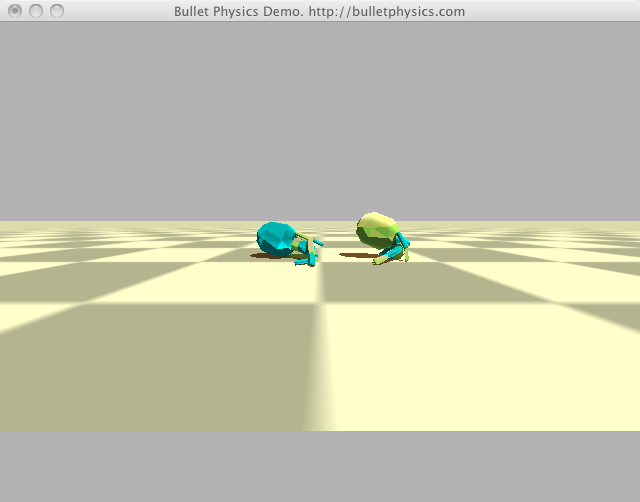
\includegraphics[width=0.48\textwidth]{Fig1b}
}
\centerline{
c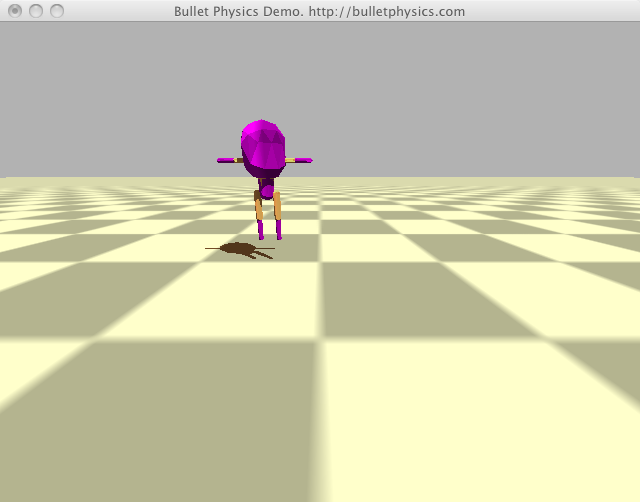
\includegraphics[width=0.48\textwidth]{Fig2}
d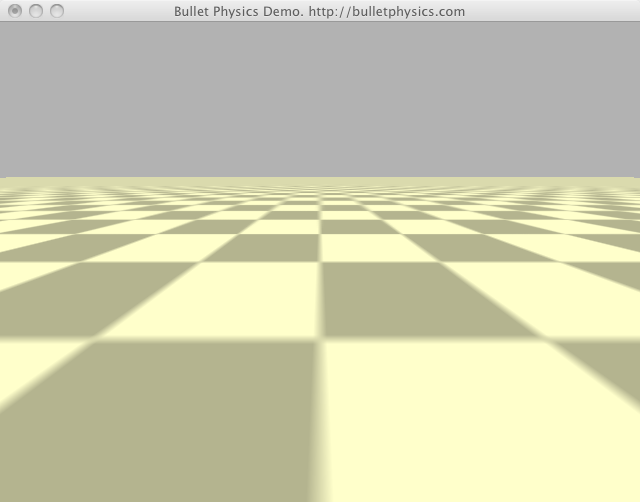
\includegraphics[width=0.48\textwidth]{Fig1d}
}
\caption{
Successful compilation and execution of the RagdollDemo program should produce \textbf{a}.
Changing the radii of the ragdoll's head should produce \textbf{b}.
Commenting out the simulation step and one ragdoll should produce \textbf{c}. 
Re-enabling the simulation and removing the final ragdoll should produce \textbf{d}.}
\label{Fig}
\end{figure}

\end{document} 
